Ante la imposibilidad de realizar la carga inalámbrica se tuvo una reunión con el cliente para discutir el proceder. El cliente indicó que el dato principal que se requiere del ave es la posición. Para la obtención de datos de la trayectoria del ave se propuso el esquema que se explica a continuación.

\Subsubsubsection{Módulos del Sistema de Seguimiento}
La propuesta se basa en cuatro partes: la mochila en el ave, las bases de seguimiento, la base principal de seguimiento y la comunicación de esta con la base del nido. 
\begin{figure}[H]
	\centering
	\begin{subfigure}{0.5\textwidth}
    	\centering
    	\includegraphics[width=\linewidth, page=1]{ImagenesFactibilidad/beacon}
    	\caption{Base de seguimiento.}
    	\label{fact:seguimiento}
    \end{subfigure}\hfill
    \begin{subfigure}{0.5\textwidth}
    	\centering
    	\includegraphics[width=\linewidth, page=2]{ImagenesFactibilidad/beacon}
    	\caption{Base principal de seguimiento.}
    	\label{fact:seguimientomain}
    \end{subfigure}	\\
    \begin{subfigure}{0.5\textwidth}
    	\centering
    	\includegraphics[width=\linewidth, page=3]{ImagenesFactibilidad/beacon}
    	\caption{Base Nido.}
    	\label{fact:nido}
    \end{subfigure}\hfill
    \begin{subfigure}{0.5\textwidth}
    	\centering
    	\includegraphics[width=\linewidth,page=4]{ImagenesFactibilidad/beacon}
    	\caption{Mochila.}
	\label{fact:beacon}
    \end{subfigure}
	\caption{Elementos ilustrativos de los módulos del sistema de seguimiento.}
	\label{fig:componentes_beacon_ilustrativo}
\end{figure}

\Subsubsubsection{Mochila}
Para la propuesta de la mochila, se llegó a la conclusión de que utilizar GPS es muy costoso en materia de energía, peso y dimensiones. Es por esto que tomó un camino alternativo, recomendando la tecnología de \textit{beacon Bluetooth}.

Se toma como ejemplo el modelo de \textit{beacon} EMBC22, cuyas dimensiones son útiles para la aplicación deseada, dado que miden $30 \ mm$ de diámetro y $10 \ mm$ de altura. Junto a la batería se llega a un peso de 10 gramos, cumpliendo así con los requerimientos de dimensiones y de peso estipulados.

La característica más notable del \textit{beacon} es que permite mandar paquetes personalizables por \textit{Bluetooth} 5.0 a bases receptoras para informar su presencia. A partir estas se puede obtener la ubicación. Además este dispositivo soporta un amplio rango de temperaturas y cuenta con un grado de protección IP-64.

Para garantizar el funcionamiento durante todo el período del estudio se calcula una vida útil de la batería\footnote{Para calcular la vida útil de la batería se utiliza la calculadora de vida útil del proveedor del \textit{beacon}.}. Con un rango de detección de hasta 200 metros y un microcontrolador con acelerómetro y \textit{firmware} personalizable, se obtiene un valor de 4 años.
\begin{figure}[H]
	\centering
	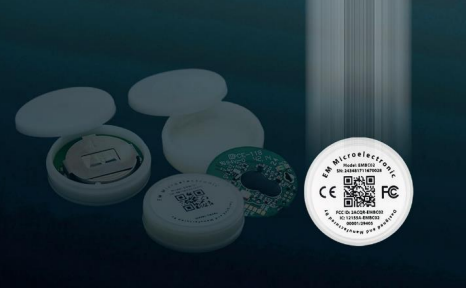
\includegraphics[width=0.7\linewidth]{ImagenesFactibilidad/beaconpic}
	\caption{Beacon EMBC22.}
	\label{fig:beacon}
\end{figure}

\Subsubsubsection{Base de Seguimiento}
Las bases de seguimiento consisten en una red de módulos receptores esparcidos por el bosque a una distancia de aproximadamente 30 metros entre sí.
Además, se hicieron las siguientes recomendaciones:
\begin{itemize}
	\item Comunicación \textit{Bluetooth} 5.0 para el \textit{beacon} acorde al estándar, con la finalidad de poder triangular su posición.
	\item Uso de red Lora o \textit{Bluetooth} 5.0 para la comunicación entre bases de seguimiento de ser necesario y con la base principal de seguimiento para reporte de datos.
	\item Uso de paneles solares y baterías para lograr independencia de la red eléctrica.
\end{itemize}
\begin{figure}[H]
\centering
	\begin{subfigure}{0.5\textwidth}
    	\centering
    	\includegraphics[width=\linewidth,page=5]{/ImagenesFactibilidad/beacon}
  		\caption{Ubicación de bases de seguimiento.}
  		\label{fig:sfig1}
    \end{subfigure}\hfill
    \begin{subfigure}{0.5\textwidth}
    	\centering
    	\includegraphics[width=\linewidth,page=6]{/ImagenesFactibilidad/beacon}
  		\caption{Triangulación de posición.}
  		\label{fig:sfig2}
    \end{subfigure}
	\caption{Elementos ilustrativos de los módulos del sistema de seguimiento.}
	\label{fig:componentes_beacon}
\end{figure}

\Subsubsubsection{Base Principal de Seguimiento}
La base principal de seguimiento junta toda la información de las demás centrales. Se considera la existencia de repetidores, los cuales son empleados para la señal del módulo principal. Esto permite extender la distancia en el caso de que la red receptora se encuentre fuera de alcance de la principal.

Dicha base también debe contar con independencia de la red eléctrica, y debe poder comunicarse con la del nido mediante \textit{Bluetooth}. El propósito de esta comunicación es el enviar un set de datos del ave una vez por día.

\Subsubsubsection{Propuesta de Valor Aumentada}
Se destaca que, al realizar el diseño sugerido, aumenta con creces la modularidad del producto final. Con la red de receptores desplegada, es posible escalar el sistema para más de un animal a la vez. Esto es posible simplemente con utilizar un \textit{beacon} en las especies que se deseen seguir. 

Debido al nivel de configuración que estos poseen, se puede distinguir a los distintos dispositivos entre sí, creando así un bosque inteligente para el seguimiento de toda su fauna.
